\subsection{$k$-NN algorithm}

The \textbf{k-nearest neighbors algorithm} (k-NN) is a non-parametric method used for regression and classification. 

Throughout this report we'll be using the k-NN algorithm to solve a classification problem. In k-NN classification, the output is a class membership. An observation will be assigned to the class most common among its $k$ nearest neighbors, with $k$ being an integer, in other words, an observation is classified by a majority vote of its neighbors.

As most classification algorithms, it has two main steps (training and prediction). The training step only consists in locally storing all the available observations, leaving all the computation to be carried out in the prediction step. This is often referred to as instance-based learning or lazy learning. The k-NN algorithm is among the simplest algorithms of machine learning.

A useful technique to improve performance can be to assign weight to each neighbor's contribution, so that nearer neighbors contribute more than distant ones.
\begin{figure}[b]
	\centering
	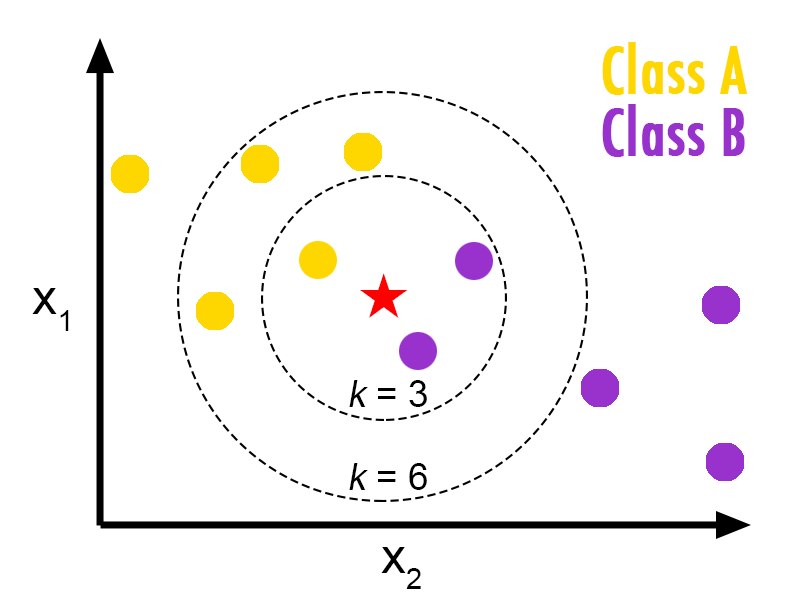
\includegraphics[width=0.42\textwidth]{Knn-introduction}
	\caption{2D algorithm visualization example}
	\label{fig:knn-introduction}
\end{figure}

\subsection{Confusion matrix terminology}

A confusion matrix table is a table often used to describe the performance of a classification model on a set of data for which true values are known. The confusion matrix itself is relatively simple to understand, but the related terminology might be confusing \cite{confmat-terminology}.
\begin{figure} % binary confusion matrix \label{fig:conf_mat}
	\centering
	\setlength{\arrayrulewidth}{0.5mm}
	\renewcommand{\arraystretch}{1.3}
	\newcommand{\colorcell}{\cellcolor{lightgray}}
	% if using array.sty, it might be a good idea to tweak the value of
	% \extrarowheight as needed to properly center the text within the cells
	\setlength\extrarowheight{0.5pt}
	\begin{tabular}{r|c|c|}
		           & predicted YES & predicted NO  \\ \hline
		actual YES & \colorcell TP & \colorcell FN \\ \hline
		actual NO  & \colorcell FP & \colorcell TF \\ \hline
	\end{tabular}
	\caption{Binary confusion matrix. TP = true positive, TN = true negative, FN = false negative, FP = false positive.}
	\label{fig:conf_mat}
\end{figure}

The basic terms are:
\begin{itemize}
	\item True positives (TP): actual and predicted outcome is positive.
	\item True negatives (TN): actual and predicted outcome is negative.
	\item False positives (FP): prediction is positive, but actual value is negative. Also known as \textit{type I error}
	\item False negatives (FN): prediction is negative, but actual value is positive. Also known as \textit{type II error}
\end{itemize}

Using the 4 previous terms, we can compute several rates that helps us evaluate the performance of a classifier.
\begin{itemize}
	\item Accuracy: overall, how often is the classifier correct.
	$$ \frac{TP + TN}{\text{total}} $$
	\item Misclassification rate: overall, how often is the classifier wrong.
	$$ \frac{FP + FN}{\text{total}} = 1 - \text{accuracy} $$
	\item \textbf{Sensitivity} or \textbf{recall}: Also known as true positive rate. When it is actually YES, how often does it predict YES.
	$$ \frac{TP}{TP + FN} $$
	\item \textbf{Specificity}: Also known as true negative rate. When it is actually NO, how often does it predict NO.
	$$ \frac{TN}{TN + FP} $$
	\item \textbf{Precision}: When it predicts YES, how often it is correct.
	$$ \frac{TP}{TP + FP} $$
	\item \textbf{F1 score}: Harmonic (weighted) average of the precision and recall where F1 reaches its best value at 1 and worst at 0. 
	$$ 2 \, \frac{\text{precision} \cdot \text{recall}}{\text{precision} + \text{recall}} $$
\end{itemize}

Although a binary confusion matrix was used to introduce the previous concepts, it can be generalized to multi-class scenarios since every confusion matrix can be decomposed into multiple binary matrices using a \textit{one-vs-all} approach. Thus, for multi-class problems we'll compute rates per class.